\documentclass[journal,12pt,onecolumn]{IEEEtran}
\IEEEoverridecommandlockouts
\usepackage[margin=0.75in]{geometry}

% defining the \BibTeX command - from Oren Patashnik's original BibTeX documentation.
\def\BibTeX{{\rm B\kern-.05em{\sc i\kern-.025em b}\kern-.08emT\kern-.1667em\lower.7ex\hbox{E}\kern-.125emX}}

%%%%%%%%%%%%%%%%%%%%%%%%%%%%%%%%%%%%%%%%%%%%%%%%%%
%%%%%%%%%%%%%%%%%%%%%%%%%%%%%%%%%%%%%%%%%%%%%%%%%%
%%%% PACKAGES.
%\usepackage[toc,page]{appendix}
%\usepackage{multirow}
%% \input{plots/latex_plot/macros_plots.tex}
%\newtheorem{Definition}{Definition}
%\newenvironment{definition}[1][Definition]{\begin{trivlist}
%\newcommand{\listappendixname}{List of Appendices}
%\newcommand{\myappendices}[1]{%
%\addcontentsline{app}{myappendices}{#1}\par}
\usepackage{amsmath}
\usepackage{amsfonts}
\usepackage{amssymb}

%\usepackage{multicol}
\usepackage{paralist}
%% plots, diagrams
\usepackage{float}
\usepackage{tikz}
\usepackage{comment}
%%\input{settings-ACM}
%%\usepackage{amsfonts,latexsym}
%%\usepackage{amsthm}
%%\usepackage{amsmath}
%%\usepackage{amssymb}
%%\usepackage[utf8]{inputenc}
%%\usepackage{caption}
%%\usepackage{verbatim}
%%\usepackage{resizegather}
%%\usepackage{appendix}
\usepackage{graphicx,pifont,color}
%\usepackage{algorithm}
%\usepackage{algpseudocode}
\usepackage{hhline}
%\usepackage{cleveref}
%\usepackage{lhelp}
\usepackage{url}
\usepackage[hidelinks]{hyperref}
%\usepackage{fancyvrb}
%\usepackage{lipsum}
%\usepackage{pstricks,pst-node,pst-grad,pst-plot}
\usepackage{multirow}
%\usepackage[final]{pdfpages}
%\usepackage{subcaption}

%%page specific style
%\usepackage{afterpage}

\usepackage{pgfplots}
\pgfplotsset{compat=1.10}
\usetikzlibrary{positioning,calc}
\usetikzlibrary{arrows.meta,chains,decorations.pathreplacing,scopes,positioning}
\usetikzlibrary{calc,shapes.multipart,chains,arrows}
\usepackage{lhelp}
\usepackage{listings}
%\usepackage{float}
\usepackage{xcolor,colortbl}
\usepackage{tcolorbox}

\usepackage{mathtools}
\usepackage{bm}
\usepackage{esvect}

%%%%%%%%%%%%%%%%%%%%%%%%%%%%%%%%%%%%%%%%%%%%%%%%%%
%%%%%%%%%%%%%%%%%%%%%%%%%%%%%%%%%%%%%%%%%%%%%%%%
\newtheorem{corollary}{Corollary}
\newtheorem{theorem}{Theorem}
\newtheorem{lemma}{Lemma}
\newtheorem{problem}{Problem}
\newtheorem{definition}{Definition}
\newtheorem{proposition}{Proposition}
\newtheorem{notation}{Notation}
\newtheorem{example}{Example}
\newtheorem{hypothesis}{Hypothesis}
\newtheorem{observation}{Observation}
\newtheorem{remark}{Remark}
\newtheorem{consequence}{Consequence}
\newtheorem{heuristic}{Heuristic}
\newenvironment{Proof}{ {\noindent} {\sc Proof} $\rhd$}{$\lhd$}

%%%%%%%%%%%%%%%%%%%%%%%%%%%%%%%%%%%%%%%%%%%%%%%%%%
%%%%%%%%%%%%%%%%%%%%%%%%%%%%%%%%%%%%%%%%%%%%%%%%%%
%%%% MATH SYMBOLS.
\def\N{\mbox{${\mathbb N}$}}
\def\Q{\mbox{${\mathbb Q}$}}
\def\R{\mbox{${\mathbb R}$}}
\def\Z{\mbox{${\mathbb Z}$}}

%%%%%%%%%%%%%%%%%%%%%%%%%%%%%%%%%%%%%%%%%%%%%%%%%%
%%%%%%%%%%%%%%%%%%%%%%%%%%%%%%%%%%%%%%%%%%%%%%%%%%
%%%% TOOLS AND ALGORITHMS.
\newcommand{\cupti}{\mbox{\sc CUPTI}}
\def\cuda{\mbox{\sc CUDA}}
\newcommand{\MWP}{\mbox{${\rm MWP}$}}
\newcommand{\CWP}{\mbox{${\rm CWP}$}}
\def\mwpcwp{\mbox{MWP-CWP}}
\newcommand{\nvcc}{\mbox{\sc nvcc}}
\newcommand{\nvprof}{\mbox{\sc nvprof}}
\newcommand{\dimThree}{\mbox{\texttt{dim3}}}

\def\cilk{\mbox{\sc Cilk}}
\def\cilkview{\mbox{\sc Cilkview}}
\def\cilkplus{\mbox{\sc CilkPlus}}
\def\openmp{\mbox{\sc OpenMP}}
\def\openmpc{\mbox{\sc OpenMPC}}
\def\openmptasks{\mbox{\sc OpenMP Tasks}}
\def\tbb{\mbox{\sc TBB}}
\def\meta{\mbox{\sc Meta\-Fork}}

%\def\opencl{\mbox{\sc OpenCL}}
\def\openacc{\mbox{\sc OpenACC}}
\def\ppcg{\mbox{\sc PPCG}}
\renewcommand{\P}{\mbox{\sf P}}
\newcommand{\MMM}{MCM}
\newcommand{\K}{\mbox{\sf K}}
%\newcommand{\blockcomment}[1]{}

%%%%%%%%%%%%%%%%%%%%%%%%%%%%%%%%%%%%%%%%%%%%%%%%%%
%%%%%%%%%%%%%%%%%%%%%%%%%%%%%%%%%%%%%%%%%%%%%%%%%%
%%%% PROOFREADING UTILS.

\newcommand{\hidetext}[1]{\mbox{ \ }}
\newcommand{\todo}[2]{{{\textcolor{red}{ #1}}}\footnote{ {\textcolor{blue}{ #2}} }}
\newcommand{\fixed}[2]{#1}
\newcommand{\reworked}[1]{{{\textcolor{orange}{ #1}}}}

%%%%%%%%%%%%%%%%%%%%%%%%%%%%%%%%%%%%%%%%%%%%%%%%%%
%%%%%%%%%%%%%%%%%%%%%%%%%%%%%%%%%%%%%%%%%%%%%%%%%%
%%%% COLORS
\definecolor{wp}{rgb}{0.129,0.478, 0.678}
%\definecolor{wp}{rgb}{0.26,0.55, 0.79}
%\definecolor{wpbright}{rgb}{0.192, 0.439, 0.561}\\
%\definecolor{wpbright}{rgb}{0.43, 0.43, 0.43}
%\definecolor{wp}{rgb}{0.19, 0.45, 0.66}
\definecolor{wpbright}{rgb}{0.26,0.55, 0.79}
\definecolor{yellowBright}{HTML}{FFD247}
\definecolor{orangeBright}{HTML}{FF7E47}
\definecolor{gray1}{HTML}{CEDBE1}
\definecolor{gray2}{HTML}{DDE6EA}
\definecolor{gray3}{HTML}{E3E6EB}
\definecolor{darkblue1}{HTML}{2375B9}%{0A599B}
\definecolor{darkblue2}{HTML}{3D577A}
\definecolor{lightblue1}{HTML}{65A4D9}
\definecolor{lightblue2}{HTML}{94C3E9}
\definecolor{red1}{HTML}{E4001B}
\definecolor{red2}{HTML}{8F2831}
\definecolor{lime1}{HTML}{AEBD63}
\definecolor{navy}{HTML}{000063}
\definecolor{purple1}{HTML}{8F2831}
\definecolor{contrast}{HTML}{CE0000}
\definecolor{positive}{HTML}{0D900F}
\definecolor{negative}{HTML}{FF0000}

%%%%%%%%%%%%%%%%%%%%%%%%%%%%%%%%%%%%%%%%%%%%%%%%%%
%%%%%%%%%%%%%%%%%%%%%%%%%%%%%%%%%%%%%%%%%%%%%%%%%%
%%%% COMMENTED
%%\newcommand{\blockcomment}[1]{}
%%\newtheorem{corollary}{Corollary}
%%\newtheorem{theorem}{Theorem}
%%\newtheorem{lemma}{Lemma}
%%\newtheorem{problem}{Problem}
%%\newtheorem{definition}{Definition}
%%\newtheorem{proposition}{Proposition}
%%\newtheorem{notation}{Notation}
%%\newtheorem{example}{Example}
%%\newtheorem{hypothesis}{Hypothesis}
%%\newtheorem{observation}{Observation}
%%\newtheorem{remark}{Remark}
%%\newtheorem{consequence}{Consequence}
%%\newenvironment{Proof}{ {\noindent} {\sc Proof} $\rhd$}{$\lhd$}
%\newcommand{\hidetext}[1]{\mbox{ \ }}
%\newcommand{\todo}[2]{{{\textcolor{red}{ #1}}}\footnote{ {\textcolor{blue}{ #2}} }}
%\newcommand{\fixed}[2]{#1}
%\newcommand{\reworked}[1]{{{\textcolor{orange}{ #1}}}}

%%\lstset { %
%%	language=C,
%%	backgroundcolor=\color{black!5}, % set backgroundcolor
%%	basicstyle=\footnotesize,% basic font setting
%%	belowcaptionskip=1\baselineskip,
%%	breaklines=true,
%%	frame=L,
%%	xleftmargin=\parindent,
%%	showstringspaces=false,
%%	basicstyle=\footnotesize\ttfamily,
%%	keywordstyle=\bfseries\color{green!40!black},
%%	commentstyle=\itshape\color{purple!40!black},
%%	identifierstyle=\color{blue},
%%	stringstyle=\color{orange},
%%	numbers=left,
%%	stepnumber=1,
%%}
%%%
%%\usepackage{booktabs}
%%%
%%\setlength{\aboverulesep}{0pt}
%%\setlength{\belowrulesep}{0pt}

%
%\newcolumntype{a}{>{\columncolor{gray1}}c}




%%%%%%%%%
% Macros for proofreading
%%%%%%%%%
\newcommand{\toremove}[1]{\textcolor{red}{#1}}
\newcommand{\removed}[1]{}

\usepackage{booktabs}
\usepackage{graphicx}
\usepackage{caption}
\usepackage{hyperref}
\hypersetup{
	colorlinks=true,
	linkcolor=blue,
	filecolor=magenta,      
	urlcolor=blue,
}
\urlstyle{same}
\usepackage{listings}
\usepackage{xcolor}

\definecolor{codegreen}{rgb}{0,0.6,0}
\definecolor{codegray}{rgb}{0.5,0.5,0.5}
\definecolor{codepurple}{rgb}{0.58,0,0.82}
\definecolor{backcolour}{rgb}{0.95,0.95,0.92}

\lstdefinestyle{mystyle}{
	backgroundcolor=\color{backcolour},   
	commentstyle=\color{codegreen},
	keywordstyle=\color{magenta},
	numberstyle=\tiny\color{codegray},
	stringstyle=\color{codepurple},
	basicstyle=\ttfamily\footnotesize,
	breakatwhitespace=false,         
	breaklines=true,                 
	captionpos=b,                    
	keepspaces=true,                 
	numbers=left,                    
	numbersep=5pt,                  
	showspaces=false,                
	showstringspaces=false,
	showtabs=false,                  
	tabsize=2
}

\lstset{style=mystyle}

\makeatletter
\DeclareRobustCommand*\cal{\@fontswitch\relax\mathcal}
\makeatother

\makeatletter
\def\endthebibliography{%
	\def\@noitemerr{\@latex@warning{Empty `thebibliography' environment}}%
	\endlist
}
\makeatother




\title{
Galaxy Morphological Classification with Convolutional Neural Network\\}


\author{
\IEEEauthorblockN{Klay Kulik\IEEEauthorrefmark{1},
Deepak Sharma\IEEEauthorrefmark{2} and
Linxiao Wang\IEEEauthorrefmark{2}}\\
\IEEEauthorblockA{\IEEEauthorrefmark{1}Department of Physics and Astronomy, \IEEEauthorrefmark{2}Department of Computer Science}\\
Email: kkulik2@uwo.ca, dsharm55@uwo.ca, lwang739@uwo.ca
}

%reducing spacing after float
\setlength\textfloatsep\baselineskip
%%%%%%%%%%%%%%%%%%%%%%%%%%%%%%%%%%%%%
\begin{document}

\maketitle

\begin{abstract}
In this project, the problem of galaxy morphological classification into two main categories is discussed, where the input data contain five bands (u, g, r, i and z) instead of the typical three channel (RGB) images. 
The data used came from the Sloan Digital Sky Survey and the Galaxy Zoo project.
Logistic Regression was first performed as a baseline on on 10000 randomly sampled galaxies, which gave a testing accuracy of $58\%$. 
A Convolutional Neural Network with five convolution layers was then built, and it classified with an accuracy of $98.5\%$ using roughly 18000 training data of each type. 
Logistic Regression and the CNN are compared, with discussion on further improvements such as fine tuning the CNN.
Assumptions that the crowdsourced data are correctly classified are reviewed, and applications of a functional CNN are given. The full report and all supplemental scripts are publicly available on \href{https://github.com/klaykulik/galaxyCNN}{GitHub}


\end{abstract}

\section{Introduction}
\label{sec:intro}
Motivate the problem and the general approaches you will use to solve it. Explain in enough detail so that a non-expert can understand why the subject-area problem is important and how you propose to solve it.

\subsection{Motivation}
Galaxies have morphology that can be split into two main categories: spiral and elliptical. 
The differences between them are fairly obvious from images: spiral galaxies are disk shaped and have curved arms extending out from the centre, while elliptical galaxies are shaped like an three dimensional blob that is brighter in the middle. 

\begin{figure}[h]
	\centering
	\captionsetup{justification=centering}
	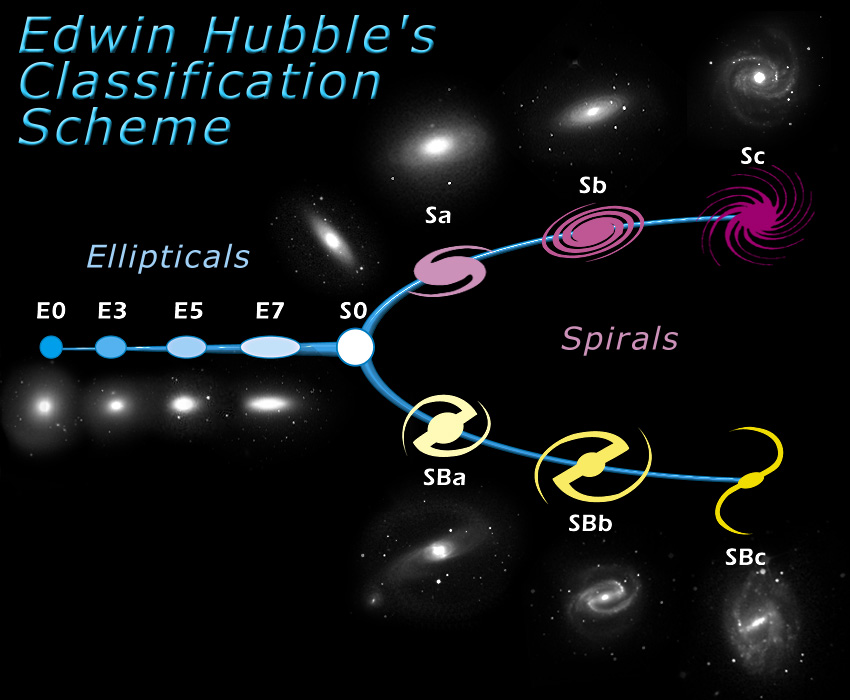
\includegraphics[scale=0.7]{Figures/TuningFork.jpg}
	\caption{Edwin Hubble's 'Tuning Fork' classification scheme. Galaxies are classified into two main categories, spiral and elliptical, with further sub-classifications representing minute changes \cite{TuningFork}.}
	\label{fig:tuningfork}
\end{figure}


There are many more differences between the two galaxy morphologies that are not as glaringly.  
For example, Spiral galaxies tend to be bluer than their elliptical cousins. 
Dense spiral arms are the birthplace of new stars, which excite gas around them and cause it to glow a blue colour. 
Elliptical galaxies lack the gas and dust required to form new stars, and therefore tend to be redder. 
When two galaxies of any type collide, they eventually form a large elliptical galaxy. 
Elliptical galaxies are much more common near the centre of galaxy clusters for this reason, and can be many times larger than their spiral counterparts.
Classifying galaxies based on their morphology therefore has a large impact on research in many fields of astronomy, including things from galactic dynamics to the age of the Universe!

Humans can easily distinguish between the two forms given the collected data is high enough resolution. 
There is one major problem in this field of research that is rather unexpected - we have too much data available to look through and separate! 
The Sloan Digital Sky Survey is one of the newer collection surveys that is starting to monopolize the field. SDSS has a list of over 200,000,000 individual galaxies across more than one third of the night sky\cite{SDSS}!

\subsection{Approach}
This is where data science comes in - a neural network trained to classify images into these categories would be extremely useful to many astronomers. 
A convolutional neural network (CNN) should be able to identify galaxies much faster than humans, with comparable accuracy.












 
\section{Data}
\label{sec:data}
\subsection{Data Source}
\label{sec:data_source}
The data we used for this project came from the Sloan Digital Sky Survey (SDSS) Data Release (DR)7~\cite{abazajian2009seventh}, and the Galaxy Zoo (GZ) project first data release~\cite{lintott2010galaxy}. 
SDSS is a major multi-spectral imaging and spectroscopic redshift survey using a dedicated wide-field 2.5 m telescope located at Apache Point Observatory (APO) near Sacramento Peak in Southern New Mexico.
DR7 contains five-band photometry for 357 million distinct objects~\cite{abazajian2009seventh}. 
The GZ project collected simple morphological classifications of nearly 900,000 galaxies drawn from SDSS DR7, contributed by hundreds of thousands of volunteers~\cite{lintott2010galaxy}. 

We took the galaxy names and classifications from the GZ database, and searched SDSS for the corresponding images. For each galaxy five FITS files are provided by SDSS.
The SDSS images are unique in that the data is stored in five bands (`ugriz') instead of the typical three channels (RGB). 
`ugriz' channels are also absolute, rather than relative, meaning that instead of ranging from 0 to 255 the pixels have an integer greater than zero which represents the energy coming from that specific region in space. 
This is so the actual intensity of the galaxy in a specific band can be extracted in order to calculate galaxy mass and composition.


\begin{figure}[h!]
	\centering
	\captionsetup{justification=centering}
	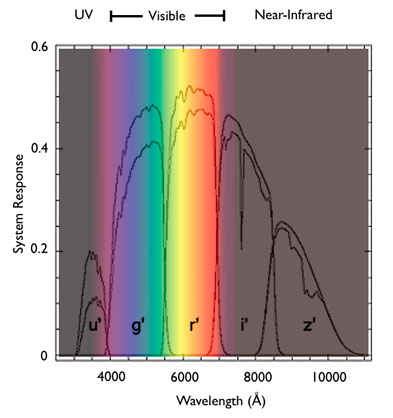
\includegraphics[scale=0.5]{Figures/filters.jpg}
	\caption{The `ugriz' filter schematic with a colour spectrum plotted on top.}
	\label{fig:filters}
\end{figure}



\subsection{Pre-processing}
Since the classifications in GZ are from crowdsourcing, we only used the data entries that
have high confidence classifications. We choose galaxies with debiased probability (given in~\cite{lintott2010galaxy}) greater than 0.985 for spiral galaxies, and 0.926 for elliptical galaxies, respectively. 
We choose these thresholds to ensure that: (i) the galaxies used for training the neural network have highly accurate classifications; and (ii) the number of data for both classes in the training and test sets are balanced~\cite{khan2019deep}. We obtained 19306 and 18811 galaxies for spiral and elliptical respectively. 

The data we got from SDSS are in Flexible Image Transport System (FITS) format. 
Each FITS file contains a header part and a data part. We removed the header part and resized the images to $200 \times 200$ pixels. As we discussed in Section~\ref{sec:data_source}, `ugriz' covers a broader band than RGB images. Common ways to map `ugriz' files to RGB images would take 3 or 4 channels (out of 5) of `ugriz', and do a linear transformation on them, thus would definitely lose some information. 
In order to keep a more complete data for each galaxy we used `ugriz' files rather than RGB images as the input to our classifier. Figure~\ref{fig:ugriz} shows the gray-scale images of the u, g, r, i and z band photometry of a spiral galaxy as well as the RGB image of the same galaxy. We can see that there is information on each band but the RGB image only uses 3 or 4 of them which would cause information loss.

\begin{figure}[h]
	\centering
	\captionsetup{justification=centering}
	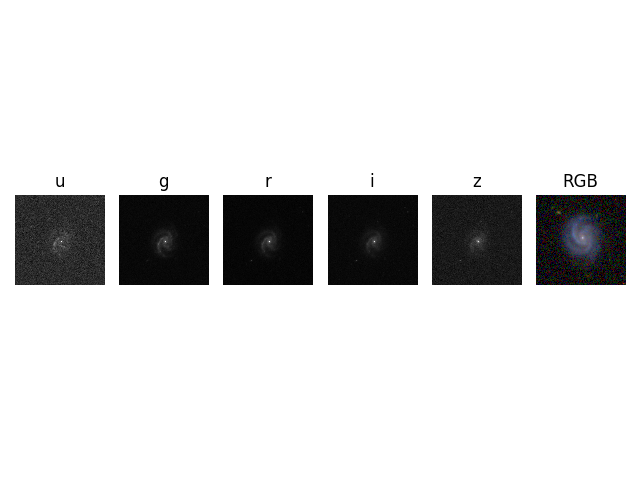
\includegraphics[trim={0 4cm 0 4cm},clip]{Figures/ugriz_vs_rgb.png}
	\caption{The `ugriz' images and the RGB image of the same galaxy.}
	\label{fig:ugriz}
\end{figure}


\section{Method}
\label{sec:method}
\subsection{Logistic Regression}
Baseline model

\subsection{Deep Learning Model - CNN}

\begin{figure}[h]
	\centering
	\captionsetup{justification=centering}
	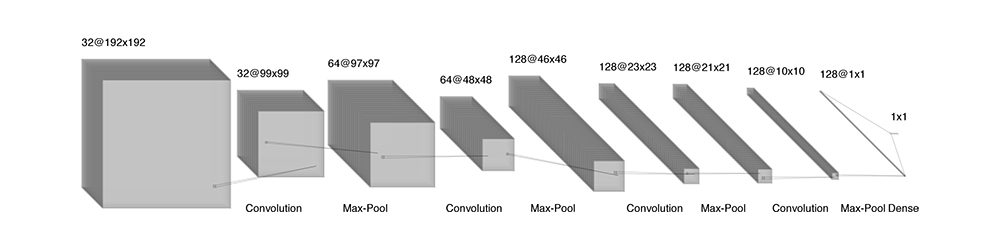
\includegraphics[width=\columnwidth]{Figures/CNNArchitecture.jpg}
	\caption{Architecture of the CNN model}
	\label{fig:cnnarch}
\end{figure}

Deep Learning has achieved significant results and a huge improvement in visual detection and recognition with a lot of categories. Raw data images are used by deep learning as input without the need of expert knowledge for optimization of segmentation parameter or feature design. We used open source software stacks for our project. The deep learning APIs used are Keras and Tensorflow. The proposed architecture of the deep network for the morphological classification is illustrated in detail in Figure~\ref{fig:cnnarch}. It consists of 15 layers, made up of 5 main layers for features extraction, followed by two principle fully connected layers for classification. The first layer is the input layer. Every main layer is further made of one convolutional layer with the Rectified Linear Unit(ReLU) as the nonlinear activation function and a max pooling layer at the end for subsampling. The first fully connected layer has 128 neurons with ReLU activation function, while the last fully connected layer has one neuron and uses a sigmoid to obtain class memberships. Visualizing the feature extraction and classification layers in the proposed deep neural architecture will give a better understating. In the main layers, features are extracted and the patterns identified become more complex as we go deeper into the network. CNNs are generally used for image classification but they are also very useful for finding patterns in any data that can benefit from filters. Using a 5 channel raw input is not typical when employing CNNs but since the image data(RGB) for the galaxy is a subset of the wavelength range of the 5 channels a CNN is very well suited for this classification task. This becomes more apparent with the results(accuracy) of the model.
\section{Results}
\label{sec:res}
Figure~\ref{fig:log_cm} shows the confusion matrix of the logistic regression model we discussed in Section~\ref{sec:log}. Among the 1000 testing data, 526 are spiral and 474 are elliptical. The accuracy of this model is 58.9\%, the precision is 55.8\% and the recall is 63.7\%. We can see that the accuracy is only slightly better than a random guess that should have the accuracy of 50\%. This lead us to believe that a more complex model is needed for this problem.

\begin{figure}[h]
	\centering
	\captionsetup{justification=centering}
	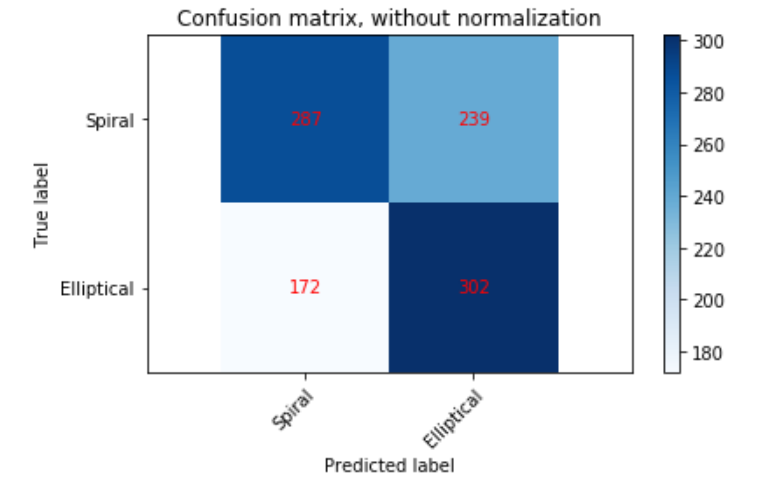
\includegraphics[width=0.6\columnwidth]{Figures/log_cm.png}
	\caption{Confusion matrix of testing data for the Logistic regression model}
	\label{fig:log_cm}
\end{figure}


\begin{figure}[h]
	\centering
	\captionsetup{justification=centering}
	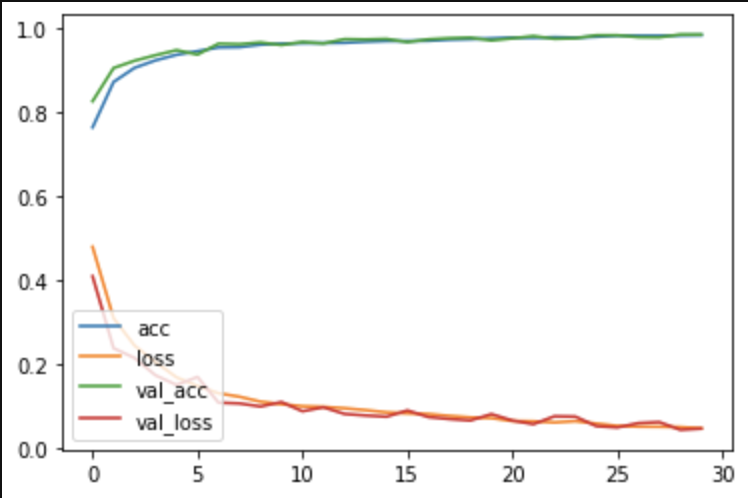
\includegraphics[width=0.4\columnwidth]{Figures/CNNMetrics.png}
	\caption{Training and validation metrics for the CNN model}
	\label{fig:cnnmetrics}
\end{figure}

Figure~\ref{fig:cnnmetrics} shows the plot of the training and validation results of CNN model we discussed in Section~\ref{sec:cnn}. 
We can see from the results that the CNN model is very promising, with a validation accuracy of 98.5\% over 30 epochs of training we can conclude that the a CNN is suitable for classifying the morphology of galaxies. With more training data and optimization of the model architecture and hypertuning the parameters the accuracy can be very well increased to over 99\%.
\section{Discussion}
\label{sec:dis}
The CNN model was trained and validated on the Galaxy Zoo data that had crowdsourced classifications, so it is possible that any bias and errors in the input data were also learned by the model. 
That being said, we could also propose that errors in the crowdsourced data are shown as misclassifications in our model, and our model is perfectly classifying the data, however unlikely that may seem. 
The only way to definitively find out the true accuracy that our model has when classifying galaxy morphology would be to manually classify all of the galaxies and compare the results. 
It would be interesting to compare the same model with image data(RGB) extracted for the same galaxies instead of `ugriz' channels. This would tell us how useful the extra information from the `ugriz' channels is for the classification of the galaxies.
With more training data and visualization of the weights at every layer we should be able to get a clear idea on what the model learned.

From the results it is clear that we can employ a CNN model in practice, even though this model was only trained on a subset of the data available in GZ.
One particular example of an application of our CNN would be with the SDSS database itself. Sloan does not classify the galaxy images it produces due to the sheer volume of data, but a CNN could easily allow for classification as soon as galaxies are observed. 




\bibliographystyle{IEEEtran}
\bibliography{reference}

\begin{appendices}
	\section{}
\label{sec:appa}
\end{appendices}

\end{document}
